\cotefile{148}
\scanpage{44}
\mspage{1}
% archive sheet number: 43
\uline{Groupoïdes de Teichmüller}.

\textcircled{1} Cas topologique.

% slanted
\margin{Finalement, tant qu'on ne travaille pas au point de vue arithmétique, il semble que c'est le gros $ {\unsure{\mathscr{T}|\mathcal{T}}}^{\pm}$ qui sera le plus utilisé, \deleted{\unsure{tandis}} c'est lui qui \unsure{intervient|apparaît} dans \unsure{ici} la factorisation la plus simple $\mathscr{T}$, et le \unsure{gpde} orienté \unsure{des surfaces|s'appelle} $\mathscr{T}^{+}$.}
La variante la plus simple est
\[
\mathscr{T}_{\mathrm{top}}^{+}\quad\text{ou}\quad \mathscr{T}_{\mathrm{top}}
\]
(\uline{groupoïde de Teichmüller} \uuline{orienté} \uline{topologique}),

\uline{objets}: surfaces \uline{à bord} compactes orientées

\uline{flèches}: classes d'isotopie d'iso (conservant l'orientation)

Variante immédiate
\[
\mathscr{T}_{\mathrm{top}}^{\pm}
\]
(\uline{groupoïde de Teichmüller} \uuline{biorienté} \uline{topologique}) :
mêmes objets, flèches sont les classes d'isotopie d'homéomorphismes (ne conservant pas néc. l'orientation).

Soit $[\pm1]$ le groupoïde ayant un seul objet $e$ (par exemple $e=\unsure{\varnothing|\phi}$) et comme groupe d'autom $\pm1$. On a un morphisme de signature
\diagram{
\begin{tikzcd}[ampersand replacement=\&]
\mathscr{T}_{\mathrm{top}}^{\pm}\arrow[r,"\unsure{\chi|X}"] \& [\pm1]
\end{tikzcd}
}
% slanted
\margin{Ça ne \unsure{vaut|va}, \unsure{si on se borne|sinon se borner} à des surfaces connexes !}
dont la \uline{fibre} \deleted{\unsure{est}} (ou noyau) est $\mathscr{T}_{\mathrm{top}}^{+}=\mathscr{T}_{\mathrm{top}}$.

La variante la plus complexe est
\[
S_{*}\mathscr{T}{\unsure{D|\mathbb D}}_{\mathrm{top}}^{+}\quad\text{ou}\quad S_{*}\mathscr{T}D_{\mathrm{top}},
\]
``\uline{groupoïde de Teichmüller} \inserted{\uline{orienté},} \uline{spécial dévissé topologique}''

\scanpage{45}
% archive sheet number: 44
\deleted{On a ainsi la notion de \uline{graphe \unsure{pondéro-rigide|pondéré-rigide}} (\unsure{formalisant|formalisé} par \unsure{ex,|ex.} la structure}

\scanpage{46}
\mspage{2}
% archive sheet number: 45
\uline{objets}: Triples $(X,\widetilde{\Sigma},\deleted{\unsure{S|\delta}}R)$, avec
\margin{$X,\deleted{\unsure{\widetilde{\Sigma}}}\partial X,\Sigma,S$}
\[
\begin{aligned}
& X\ \text{surface à bord compacte orientée}\\
& \widetilde{\Sigma}\ \text{sous-variété compacte de }X\ \deleted{\unsure{\partial X|XXX}},\quad \widetilde{\Sigma}\mathrel{\unsure{\supset|>}}\partial X\\
& \deleted{\unsure{S|\delta}}R\subset\Sigma\ \deleted{\unsure{\setminus\partial X}},\ \text{partie finie}
\end{aligned}
\]
% slanted
\margin{$\widetilde{\Sigma}=\partial X\amalg\Sigma$\\On peut considérer que $R$ rigidifie, mais \unsure{non} que $R$ ``\unsure{découpe}'' $\Sigma\ldots$}
\uline{flèches}: classes d'isotopie d'homéom. conservant l'orientation

\deleted{Variante \unsure{avec}} Les composantes connexes de $\widetilde{\Sigma}\setminus\partial X$ \inserted{$=\Sigma$} \unsure{sont} les \uline{cercles de découpage}, \inserted{celles de $\partial X$ \unsure{sont} les \uline{cercles de raccord},} les éléments de $\deleted{\unsure{S|\delta}}R$ \unsure{sont} les \deleted{\unsure{points marqués|points repères}} \uline{sommets de \deleted{\unsure{marquage|repérage}}\inserted{rigidification}}, \deleted{\unsure{(ou de rigidification)}}, \deleted{les composantes connexes de $\partial X$ sont les ``\uline{\unsure{trous}}''}. Les composantes connexes de $X$ sont les \deleted{\unsure{morceaux}}\inserted{\uline{\unsure{composants|composantes}}} de l'objet envisagé.

Variante
\[
S_{*}\unsure{\mathscr{T}|\mathcal{T}}D_{\mathrm{top}}^{\pm},\quad \text{avec}
\]
\diagram{
\begin{tikzcd}[ampersand replacement=\&]
S_{*}\mathscr{T}D_{\mathrm{top}}\arrow[r,hook,no head] \& S_{*}\mathscr{T}D_{\mathrm{top}}^{\pm}\arrow[r] \& [\pm1]
\end{tikzcd}
}
comme tantôt.

On a des sous-groupoïdes pleins
\diagram{
\(\begin{array}{cl}
\begin{gathered}
R=\unsure{\varnothing|\phi},\quad \unsure{\Sigma|\bar{\Sigma}}=\deleted{\unsure{\partial X}}\varnothing\\
\deleted{\unsure{\Sigma=\varnothing}}
\end{gathered}
 &\mathscr{T}_{\mathrm{top}}\ \text{et}\ \mathscr{T}_{\mathrm{top}}^{\pm}\\
\begin{gathered}
\Sigma=\deleted{\unsure{\varnothing}}\partial X\\
R\ \text{quelconque}
\end{gathered}
 & S_{*}\mathscr{T}_{\mathrm{top}}\ \text{et}\ S_{*}\mathscr{T}_{\mathrm{top}}^{\pm}\\
\deleted{\unsure{S}}R=\varnothing & \mathscr{T}\deleted{\unsure{{}_{*}}}D_{\mathrm{top}}\ \text{et}\ \mathscr{T}D_{\mathrm{top}}^{\pm}
\end{array}\)
}
(groupoïdes de Teichmüller \uline{spéciaux} \inserted{(ou \uline{rigidifiés})} (\unsure{topologiques|topologique} orienté))

(Cas pas \unsure{intéressant} je crois, sauf \deleted{pour} $\Sigma\deleted{\unsure{=}}\unsure{\ne|=}\varnothing$ également)

% slanted
\margin{$MD=$ ``modulaire'' ou Mumford-Deligne}
\deleted{\unsure{Dé}} \uline{Détermination} du $\pi_{0}(S_{*}\mathscr{T}D_{\mathrm{top}})\xrightarrow{\sim}\pi_{0}(S_{*}\mathscr{T}D_{\mathrm{top}}^{\pm})$.

On introduit les \uline{graphes} \deleted{\unsure{MD}} bipondérés

\scanpage{47}
\mspage{3)}
% archive sheet number: 46
qui forment un groupoïde \deleted{\unsure{MD}}. $\mathrm{Grbip}$ ou $(\unsure{\mathrm{Grabipond}|\mathrm{Grbipond}})$

% slanted
\margin{pas assez précis comme donnée. La pondération d'une arête doit être remplacée par celle d'un pol. comb. $\unsure{T_{a}}$ avec $\unsure{\omega(T_{a})\simeq\omega(a)}$}
Objets : graphes \inserted{finis} $(S,\vec A,\sigma,o)$ \inserted{+ structure suppl.} (pouvant avoir des sommets isolés, des boucles fermées, a fortiori plusieurs arêtes entre deux sommets, et aussi des ``\uline{arêtes} libres'' correspondant aux pts fixes de $\sigma$)

$S,\vec A$ (ens. fini\unsure{s}) \inserted{(``sommets'', ``\unsure{arcs}'')}, $\sigma:\vec A\mathbin{-}\vec A$ involution, $o:\vec A\to S$ appl. ``origine''. On se donne de plus
\margin{j'ai indiqué une pondération des sommets, mais pas des arêtes}
\figure{
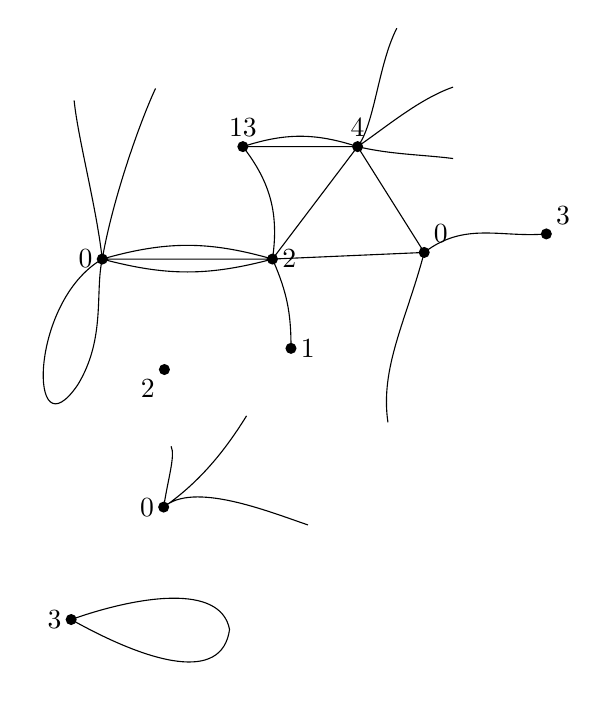
\begin{tikzpicture}[x=.94cm,y=.84cm]
\coordinate (a) at (0,0);
\coordinate (b) at (2.3,0);
\coordinate (c) at (1.9,1.7);
\coordinate (d) at (3.45,1.7);
\coordinate (e) at (4.35,.1);
\coordinate (f) at (6,.38);
\coordinate (g) at (2.55,-1.35);
\draw (a) -- (b) (a) to[bend left=16] (b) (a) to[bend right=15] (b);
\draw (a) .. controls (-1,-.65) and (-1,-3) .. (-.33,-1.9) .. controls (.05,-1.2) and (-.10,-.5) .. (a);
\draw (a) .. controls (-.08,.8) and (-.33,1.83) .. (-.38,2.4);
\draw[thin] (a) .. controls (.14,.9) and (.5,2.05) .. (.72,2.58);
\draw (b) to[bend right=23] (c) (c)--(d) (c) to[bend left=18] (d)
      (b)--(d)--(e)--(b) (b) to[bend left=12] (g);
\draw (d) .. controls (3.68,2.03) and (3.73,2.95) .. (3.98,3.49)
      (d) .. controls (3.83,1.99) and (4.28,2.42) .. (4.74,2.60)
      (d) .. controls (3.9,1.58) and (4.32,1.58) .. (4.74,1.52);
\draw (e) .. controls (4.9,.57) and (5.38,.32) .. (f)
      (e) .. controls (4.11,-.92) and (3.75,-1.64) .. (3.86,-2.47);
\foreach \p/\pos/\weight in {a/left/0,b/right/2,c/above/13,d/above/4,e/above right/0,f/above right/3,g/right/1}
  \fill (\p) circle (2pt) node[\pos] {$\weight$};
\fill (.84,-1.67) circle (2pt) node[below left] {$2$};
\coordinate (h) at (.83,-3.75);
\draw (h) .. controls (.89,-3.31) and (.99,-2.97) .. (.93,-2.83)
      (h) .. controls (1.36,-3.34) and (1.7,-2.82) .. (1.95,-2.37)
      (h) .. controls (1.23,-3.36) and (2.23,-3.81) .. (2.78,-4.02);
\fill (h) circle (2pt) node[left] {$0$};
\coordinate (k) at (-.42,-5.45);
\draw (k) .. controls (.49,-5.09) and (1.6,-4.9) .. (1.72,-5.60)
          .. controls (1.62,-6.41) and (.65,-6.12) .. (k);
\fill (k) circle (2pt) node[left] {$3$};
\end{tikzpicture}
}
\diagram{
\begin{tikzcd}[ampersand replacement=\&]
S\arrow[r,"\deleted{\unsure{g}}\,\unsure{\gamma|g}"] \& \mathbb N
\end{tikzcd}
}
(application ``genre'' ou ``poids'')
\diagram{
\begin{tikzcd}[ampersand replacement=\&]
\deleted{\unsure{\vec A|\widetilde A}}=\unsure{A_\ell|\vec A_\ell}\arrow[r,"\deleted{\unsure{\rho|p}}\,\unsure{r}"] \& \mathbb N
\end{tikzcd}
}
(application \deleted{\unsure{indice de marquage|rigidification}} ``indice de rigidification'')
\deleted{\unsure{déf.} ``\illegible{3}'' $\vec A/\sigma$ \unsure{aux faux sommets} \illegible{1} ``\unsure{vrais sommets}''}

\deleted{Ou encore, posant $\widetilde S=S\amalg A_\ell$, (identifié à l'ens de \uline{tous} les ``sommets'', ``\deleted{\unsure{vrais}}\inserted{\uline{\unsure{marqués|vrais}}}'' (i.e. $\in S$) et ``libres'' (i.e. \unsure{correspondant} aux $\unsure{a\in A_\ell}$) du graphe), l'on donne}
\diagram{
\begin{tikzcd}[ampersand replacement=\&]
\deleted{\widetilde S}\arrow[r,"\deleted{\pi}","\times"description] \& \deleted{\mathbb N}
\end{tikzcd}
}
(\uline{pondération} du graphe)

\margin{$\widetilde S=S\amalg\deleted{\unsure{\widetilde A_\ell}}A_\ell$ \deleted{\illegible{1}}}
\margin{$\widetilde A=\vec A/\sigma=A\amalg A_\ell$}
\diagram{
\begin{tikzcd}[ampersand replacement=\&]
\vec A\arrow[d,"\deleted{\unsure{\pi}}"]=
\& \underset{\vec A\setminus\vec A^\sigma}{\vec A_0}\arrow[d,"\mathrm{deg}\,2"]\amalg
\& \underbrace{\vec A_\ell}_{\vec A^\sigma}\arrow[d,"\mathrm{deg}\,1"]\\
\widetilde A= \& A\amalg \& A_\ell
\end{tikzcd}
}
\margin{Ordre d'un sommet $\,\sigma(s)=\underbrace{\sigma_\ell(s)}_{\substack{\text{correspond}\\\text{aux ``trous''}\\\text{ou cercles}\\\text{de recollage}}}+\sigma_0(s)$}

La donnée du \uline{graphe} sous-jacent à un graphe \deleted{\unsure{MD}}\inserted{bip.} revient à celle du graphe ``ordinaire'' correspondant (sans d'arêtes libres, i.e. où $\sigma$ opère sans pts fixes), i.e.
\[
(S,(\vec A\setminus\vec A^\sigma),\,\sigma|(\vec A\setminus\vec A^\sigma),\,o|\vec A\setminus\vec A^\sigma)),
\]
\uline{plus} un ensemble \inserted{fini} $A_\ell$ (\deleted{\unsure{sommets}}\inserted{arêtes} libres) \deleted{\unsure{ou} ``\unsure{sommets-trous}''} et une application
\[
A_\ell\longrightarrow S
\]
\uline{Flèches}\quad les iso. de telles structures

\scanpage{48}
\mspage{4)}
% archive sheet number: 47
On a un foncteur
\diagram{
\begin{tikzcd}[ampersand replacement=\&]
(*)\qquad \Gamma:\quad S_{*}{\unsure{\mathscr T|\mathcal T}}D_{\mathrm{top}}^{\pm}\arrow[r] \&
\deleted{\unsure{\mathrm{FMD}|\mathrm{GMD}}}(\mathrm{Grabipond})
\end{tikzcd}
}
qui associe à un objet \inserted{$(X,\widetilde{\Sigma},R)$} de $S_{*}\mathscr{T}\deleted{\unsure{D}}D_{\mathrm{top}}^{\pm}$ le graphe \inserted{MD} $(S,\vec A,\sigma,\deleted{\unsure{\pi}}o,\unsure{\gamma|g},\unsure{\rho|r})$ suivant :
\[
S=\pi_{0}(X\deleted{\unsure{/}}\setminus\widetilde{\Sigma})\simeq
\pi_{0}(\mathrm{Déc}(X,\widetilde{\Sigma}))
\]
\[
\begin{aligned}
\vec A={}&\text{ens des couples }(C,\deleted{\unsure{o}}\omega),\ \text{où }C\ \deleted{\unsure{\text{est un}}}\inserted{\in\pi_{0}(\widetilde{\Sigma})},\ \text{et où}\\
&\omega\in\mathrm{Or}(C)\inserted{\simeq\mathrm{rive}_{X}(C)},\ \text{soumise à la condition que si}\\
&C\in\pi_{0}(\partial X),\ \text{alors ce soit l'orientation induite}\\
&\text{i.e. la rive qui se trouve dans }X
\end{aligned}
\]
\[
\begin{aligned}
\sigma={}&\text{échange des rives (quand on a le droit d'échanger,}\\
&\text{sinon, i.e. si }C\in\pi_{0}(\partial X),\ \text{on pose }\sigma(a)=a\text{)}
\end{aligned}
\]
$\deleted{\unsure{o}}o$ : \deleted{\unsure{Détermine}} associe à $(C,\text{rive de }C)$ l'unique ``\unsure{face}'' $\in\pi_{0}(X\setminus\widetilde{\Sigma})$ qui contient cette rive
\diagram{
\begin{tikzcd}[ampersand replacement=\&]
\gamma:\ \underset{\substack{\Vert\\\pi_{0}(X\setminus\widetilde\Sigma)}}{S}\arrow[r] \& \mathbb N
\end{tikzcd}
}
- application \uline{genre} des composantes $X_{\unsure{i|1}}$.
\diagram{
\begin{tikzcd}[ampersand replacement=\&]
\deleted{\unsure{\rho}}r:\ A=\pi_{0}(\widetilde{\Sigma})\arrow[r] \& \mathbb N\ :\ C\longmapsto\mathrm{Card}(R\cap C).
\end{tikzcd}
}

Le foncteur $(*)$ \deleted{est ess. \uline{surjectif} et} \inserted{induit un \uline{iso} sur les} $\pi_{0}$ et \unsure{une|un} \unsure{surjectif|surject.} sur les $\pi_{1}$ (c'est un $0$-\uline{isomorphisme} \deleted{\unsure{)|?}}, en langage homotopique).

\deleted{\unsure{Le fonct.}}\quad

\uline{Remarques} Dans $S_{*}\mathscr{T}D_{\mathrm{top}}^{\pm}$ il y a une opération évidente de \uline{somme} \inserted{\uline{directe}}, dans \deleted{FMD}\inserted{Grabipond} aussi, et $(*)$ y commute.

\scanpage{49}
\mspage{5)}
% archive sheet number: 48
Cette opération de somme est la plus triviale parmi les opérations qu'il nous faudra expliciter et transcrire (combinatoirement) dans la suite. Notons de suite, pour $(X,\widetilde{\Sigma},R)$, donné
\[
X\ \deleted{\unsure{\text{est}}}\text{connexe}
\quad\Longleftrightarrow\quad
\Gamma\mathrm{MD}(X,\widetilde{\Sigma},R)\ \text{connexe}
\]
plus précisément
\[
\pi_{0}(X)\simeq\pi_{0}(\Gamma\mathrm{MD}(X,\widetilde{\Sigma},R))
\]
% slanted
\margin{dans ce cas formule pour le genre d'une $\alpha\in\pi_{0}(X)\simeq\pi_{0}(\Gamma)$ en termes de la pondération --- plus généralement, $\unsure{g_s}$ donné par $\Gamma$. Le \uline{genre total} est $g=\sum_{s\in S}g_{s}+c(\Gamma)$, \unsure{indice de connexion|indice de connexité} du graphe $\unsure{=\mathrm{rg}}\,H_{1}(\Gamma)$ \deleted{\unsure{\mathrm{caract.}}}}

\uline{Cas particuliers}.

a) Cas de $S_{*}{\unsure{\mathscr T|\mathcal T}}_{\mathrm{top}}^{\pm}\ \deleted{\unsure{S_{*}\mathscr{T}D_{\mathrm{top}}}}$ --- ici $\Sigma=\unsure{\varnothing|\phi}$, $\widetilde{\Sigma}=\partial X$.

Cela correspond \unsure{à ce que|au cas où} les graphes MD \deleted{qui} où \inserted{toutes les arêtes sont libres, i.e.} tous les sommets sont isolés (sauf arêtes libres) \deleted{\unsure{Le}} \inserted{Ce graphe} est donc déterminé par
\diagram{
\begin{tikzcd}[ampersand replacement=\&]
A\ (\unsure{\simeq|=} \vec A\,\unsure{=|-}\,\vec A^{\sigma})\arrow[d]\arrow[r,"\unsure{r|\rho}"]\&\mathbb N\\
S\arrow[r,"\gamma"]\&\mathbb N
\end{tikzcd}
}
Le cas de $\mathscr T_{\mathrm{top}}^{\pm}$ correspond à choisir $\rho=0$, donc la situation est donnée par
\figure{
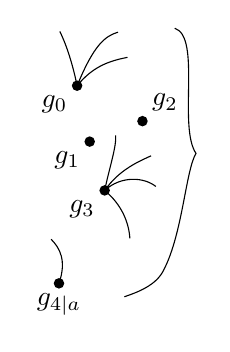
\begin{tikzpicture}[x=1cm,y=1cm]
\coordinate (a) at (.38,3); \coordinate (d) at (.73,1.67); \coordinate (e) at (.15,.49);
\draw (a) .. controls (.31,3.34) and (.22,3.57) .. (.16,3.69)
      (a) .. controls (.59,3.51) and (.73,3.63) .. (.9,3.68)
      (a) .. controls (.57,3.23) and (.76,3.31) .. (1.02,3.36);
\draw (d) .. controls (.79,1.96) and (.88,2.22) .. (.87,2.37)
      (d) .. controls (.92,1.94) and (1.17,2.04) .. (1.32,2.11)
      (d) .. controls (.94,1.86) and (1.23,1.84) .. (1.38,1.72)
      (d) .. controls (.96,1.48) and (1.04,1.24) .. (1.05,1.06);
\draw (e) .. controls (.25,.78) and (.16,.94) .. (.05,1.05);
\fill (a) circle (1.9pt) node[below left] {$g_0$};
\fill (.54,2.29) circle (1.9pt) node[below left] {$g_1$};
\fill (1.21,2.55) circle (1.9pt) node[above right] {$g_2$};
\fill (d) circle (1.9pt) node[below left] {$g_3$};
\fill (e) circle (1.9pt) node[below] {$g_{\unsure{4|a}}$};
\draw (1.62,3.73) .. controls (1.96,3.62) and (1.66,2.48) .. (1.89,2.14)
      .. controls (1.76,1.93) and (1.72,1.12) .. (1.48,.66)
      .. controls (1.39,.47) and (1.16,.38) .. (.98,.32);
\end{tikzpicture}
}
\diagram{
\begin{tikzcd}[ampersand replacement=\&]
A=\unsure{A_0|A_\ell}\arrow[d]\&\\
S\arrow[r,"\gamma"]\&\mathbb N\quad .
\end{tikzcd}
}
\deleted{type $(g,\nu)$ d'un \unsure{sommet}} Le cas d'une situation connexe ($\mathrm{card.}\,S=1$ \inserted{i.e. $S=\{s\}$}) est \deleted{\unsure{bien caractérisé par le genre}} \inserted{caractérisé} par la donnée des deux entiers $(g,\unsure{\nu|v})$ ($g=$ genre, $\nu=$ nb de trous)
\[
g=\gamma(s),\quad \unsure{\nu|\gamma}=\mathrm{card}\, A
\]

\scanpage{50}
\mspage{6}
% archive sheet number: 49
\uline{Remarque} En fait, on a un foncteur plus précis, vers une catégorie de graphes munis d'une structure où la partie $\rho$ de la pondération est \deleted{\unsure{complétée}} \inserted{\unsure{remplacée}} par une structure plus précise, à savoir \deleted{une \unsure{application}} \deleted{\unsure{une appli.}} famille
\[
\deleted{\unsure{A|\Delta}\,(\unsure{\widetilde R,\alpha,p:R\to\vec A}\ \underset{\vec A/\unsure{\sigma|\alpha}}{\Vert})}\quad (R_a)_{a\in A}
\]
% slanted
\margin{$\omega(a)\overset{\mathrm{def}}{=}\{\vec a\in\vec A\ /\ \vec a\text{ au dessus de }a\}$}
d'ensembles, et pour $\forall a\in A$, si $\omega(a)$ désigne l'ens des ``orientations'' de $a$ ($\unsure{\mathrm{card}\,\omega(a)|\mathrm{card}\,|\omega(a)|}\in\{1,2\}$), une application
\deleted{\unsure{un ensemble fini} $R$, et $p$ une application $R\longrightarrow A$ \unsure{composée}}
\diagram{
\begin{tikzcd}[ampersand replacement=\&]
\omega\longmapsto u_{\omega}:\quad\omega(a)\arrow[r] \& \mathrm{Circ}(R_{a})
\end{tikzcd}
}
ou des permutations circulaires sur $R_{a}$
\deleted{et \unsure{aussi} une \unsure{autre} application \uline{\unsure{injective}}}
\diagram{
\begin{tikzcd}[ampersand replacement=\&]
\deleted{\unsure{R/\alpha}}\arrow[r,hook,"\times"description]\&\deleted{\unsure{\vec A|\widetilde A}}
\end{tikzcd}
}
avec la condition que si $\omega,\omega'\in\omega(a)$, $\omega\ne\omega'$, alors $\deleted{u_{\omega}u_{\omega'}=\mathrm{id}_{R_{a}}}\,u_{\omega'}=u_{\omega}^{-1}$

On peut aussi considérer que la donnée supplémentaire revient à la donnée de
\diagram{
\begin{tikzcd}[ampersand replacement=\&]
\underset{\substack{\Vert\\a\mapsto\mathrm{Card}\,p^{-1}(a)}}{r:}\quad A\arrow[r]\&\mathbb N
\end{tikzcd}
}
(la ``pondération-arêtes''), et la donnée d'une famille de torseurs
\[
(R_{a})_{a\in A},\quad \deleted{\unsure{\text{avec}}}
\]
$R_a$ un torseur sous $\mathbb{Z}/r(a)\mathbb{Z}\wedge_{\{\pm1\}}^{\omega(a)}$. On associe à $(X,\widetilde{\Sigma},R)$ une telle structure supplémentaire
\[
R_{a}=R\cap\widetilde{\Sigma}_{a}\quad
(\widetilde{\Sigma}_{a}\ \text{la comp. connexe de }\widetilde{\Sigma}\
\deleted{\unsure{\text{correspondant}}}\ \text{qui correspond à } a\in A\simeq\pi_{0}(\widetilde{\Sigma})),
\]
\diagram{
\begin{tikzcd}[ampersand replacement=\&]
\deleted{\unsure{R=R(X_C)|R=R(\ast)}}\ ,\quad\deleted{R}\arrow[r,"\times"description]\arrow[d,equal]\&
\deleted{S}\arrow[d,equal]\\
\deleted{\unsure{\Gamma}}\arrow[r,"\times"description]\&\deleted{\pi_0(\widetilde{\Sigma})}
\end{tikzcd}
}
et $\omega\mapsto u_{\omega}$ défini de façon évidente.
\deleted{$p$ déduit de l'ordre circulaire sur les $R_a$}

\uline{NB} Même si $\unsure{r(\omega)|r(a)}=1$ ou $r(\omega)=2$, le fait de disposer

\scanpage{51}
\mspage{\deleted{\unsure{6}}7}
% archive sheet number: 50
d'une structure déjà orientée si $a$ est une arête libre (correspondant à un $C\in\pi_{0}(\partial X)$), ou qu'on dispose \inserted{de} l'une des deux orientations $\omega(a)$ --- dans le cas où $a$ est une arête ordinaire, indique que l'on tient en mains, pour chaque $a\in A$, un polygone combinatoire $P_a$, dont l'ens des sommets est $R_a$, et l'ens des arêtes peut se décrire \deleted{\unsure{comme}} de façon canonique en termes de $R_a,\omega_a$ et $\omega_a\longrightarrow\mathrm{Circ}(R_a)$. Il peut être plus commode de le \unsure{donner|sortir} d'emblée dans la structure, où la famille des $R_a$, serait remplacée par un \deleted{\unsure{qui serait donc un ensemble}} \uline{contour combinatoire}, i.e un ensemble de repères $\underline{\vec R}$ (plutôt ``repères de rigidification''), avec une opération de
\[
\underline{\unsure{D|\mathbb D}}_{\infty}
=\{\sigma_{0},\sigma_{1}\mid\sigma_{0}^{2}=\sigma_{1}^{2}=1\}
\]
dessus, et une application
\diagram{
\begin{tikzcd}[ampersand replacement=\&]
\underline{\vec R}\arrow[r]\&\vec A
\end{tikzcd}
}
compatible avec l'hom
\diagram{
\begin{tikzcd}[ampersand replacement=\&]
\underline D_{\infty}\arrow[r,"\unsure{\varepsilon|\epsilon}"]\&\{\pm 1\}
\end{tikzcd}
}
sur les groupes d'opérateurs, mais de plus un sous ens
\[
\underline{\vec R}_{\ell}^{+}\subset\underline{\vec R}|\,\vec A_{\ell}
\qquad
\begin{aligned}
&(\vec A_{\ell}=\text{arêtes libres,}\\
&\quad\text{correspondant aux}\\
&\quad\text{cercles de \unsure{recollement|recollage}}\\
&\quad\text{i.e. les }\in\pi_0(\deleted{\unsure{\Sigma}}\partial X))
\end{aligned}
\]
définissant une orientation des contours \unsure{correspondant|correspondants}.

\scanpage{52}
\mspage{8}
% archive sheet number: 51
On a ainsi la notion de \uline{graphe pondéré} \deleted{\unsure{rigidifié}} \inserted{\uline{à repères}}
\margin{$\unsure{r|\Gamma}$}
\diagram{
\begin{tikzcd}[ampersand replacement=\&]
\vec R_{\ell}^{+}\ \deleted{\unsure{D_{\infty}}}\subset
\underset{\sigma_0,\sigma_1}{\vec R}\arrow[r] \&
\vec A\arrow[loop right,"\sigma"]\arrow[d,swap,"o"]\&\\
\& S\arrow[r,"\gamma"]\&\mathbb N
\end{tikzcd}
}
Groupoïde (\uline{Gr.pondrep})

foncteur
\diagram{
\begin{tikzcd}[ampersand replacement=\&]
S_{*}\unsure{\mathscr T|\mathcal T}D_{\mathrm{top}}^{\pm}\arrow[r]\&(\mathrm{Gr\ pond\ rep})
\end{tikzcd}
}
qui sera importante sans doute dans l'explicitation de l'opération de ``recollement''. Il est clair en tous cas que toute \unsure{description-traduction} algébrico-combinatoire de $S\mathscr T D_{\mathrm{top}}^{\pm}$ devra permettre, pour chaque objet des \deleted{la catégorie}\inserted{groupoïdes-}paradigmes, de reconstituer (à isom. unique près) le \uline{graphe pondéré à repères} correspondant.

--- plus précisément, il faut reconstituer le foncteur canonique
\diagram{
\begin{tikzcd}[ampersand replacement=\&]
S_{*}\mathscr T D_{\mathrm{top}}^{\pm}\arrow[r]\&(\mathrm{Gr.pondrep.})
\end{tikzcd}
}
(et non seulement le foncteur à valeurs dans (Grbipond))

\uline{Opérations essentielles}

A) Opérations ``d'oubli'' ou de ``\uline{gommage}''.

\textcircled{1} \uline{Gommage de repères} À un objet $(X,\Sigma,R)$, muni en plus d'une partie $R'\subset R$, il associe $(X,\Sigma,R\setminus R')$ (gommage de $R'$).

\scanpage{53}
\mspage{9}
% archive sheet number: 52
% slanted
\margin{\scriptsize\uline{NB} Cette opération a l'air d'un \uline{affaiblissement} de structure --- mais en affaiblissant, sur une composante $C$ donnée de $\unsure{\Sigma^{+}|\widetilde{\Sigma}}$, lorsqu'on ``gomme'' \uline{tous} les repères de $C$ --- \unsure{donc} c'est au contraire plutôt dans la nature d'un renforcement de structure, --- ou plutôt, du moment qu'on se sert des $R'_C=R'\cap\unsure{C|X}$, dans les catégories topologiques, pour distinguer l'opération de gommage \unsure{et celle de} \deleted{\unsure{enlever tout}} de \unsure{sous-marquage} (cf plus bas), \unsure{à aucun|aucun de} \illegible{2} sont inverses. \unsure{Deux autres|Décrire} des \illegible{2} sont des équivalences de groupoïdes. \unsure{Alors, il faudrait|Il faudrait alors} séparer les deux cas, \unsure{pour distinguer nos} \uline{opérations de gommage essentielles} \unsure{(mieux|moyen)}, et (\unsure{qui change} \illegible{2}) \unsure{pour les} \unsure{cf} les contours.}

\uline{NB} Ayant (via un groupoïde équivalent \deleted{\unsure{de}} à description purement combinatoire) ``reconstruit'' \unsure{ou} \deleted{\unsure{proprement}} réalisé le groupoïde $S{\unsure{\mathscr T|\mathcal T}}D_{\mathrm{top}}^{\pm}$, et le foncteur
\diagram{
\begin{tikzcd}[ampersand replacement=\&]
S\mathscr T D_{\mathrm{top}}^{\pm}\arrow[r]\&(\mathrm{Gr.\ pond.\ rep})
\end{tikzcd}
}
\unsure{on aura} \deleted{\unsure{par|pas}} donc aussi \deleted{\unsure{une formulation de}} \inserted{l'équivalent de} \deleted{\unsure{de}} la donnée d'un $(X,\Sigma,R)$, muni \uline{en plus} d'une partie $R'\subset R$ --- \deleted{\unsure{d'où}} i.e. \unsure{avec} la construction d'un groupoïde \unsure{représentant}
\diagram{
\begin{tikzcd}[ampersand replacement=\&]
S_{*}\mathscr T D_{\mathrm{top}}^{\pm}\arrow[d]\&
\text{(à sous ens. marqué }R'\text{)}
\quad\begin{aligned}&\text{de sommets-}\\&\text{repères}\end{aligned}\\
S_{*}\mathscr T D_{\mathrm{top}}^{\pm}\&
\end{tikzcd}
}
Et \deleted{\unsure{donc}} il nous faudra donc \inserted{décrire} un foncteur ``gommage en $R'$''
\diagram{
\begin{tikzcd}[ampersand replacement=\&]
S_{*}\mathscr T D_{\mathrm{top}}^{\pm}
  (\underset{\text{marqué}}{\overset{\text{sous}}{\deleted{\unsure{R}}R'}})
\arrow[r,"\text{gommage de }R'"]\&{}\arrow[r]\&
S_{*}\mathscr T D_{\mathrm{top}}^{\pm}
\end{tikzcd}
}
\deleted{Cela s'exprime, sur le}
donnant lieu à un diagramme comm. de foncteurs
\diagram{
\begin{tikzcd}[ampersand replacement=\&]
S_{*}\mathscr T D_{\mathrm{top}}^{\pm}(\ldots R'\ldots)
  \arrow[rr,"\text{gommage de }R'"]\arrow[d,"\substack{\text{oubli du marquage}\\R'}"]\&
\&S_{*}\mathscr T D_{\mathrm{top}}^{\pm}\arrow[ddl]\\
S_{*}\mathscr T D\deleted{\unsure{R}}_{\mathrm{top}}^{\pm}\arrow[dr]\&
\&\\
\&(\mathrm{Gra}\deleted{\unsure{\mathrm{b}}}\mathrm{bipond})
\arrow[r]\&\substack{\text{graphes avec}\\\text{pondération}\\\text{par }\unsure{\gamma|\sigma}\text{, mais}\\\text{non par }r\text{,}}
\end{tikzcd}
}
alors qu'au niveau

\scanpage{54}
\mspage{10}
% archive sheet number: 53
des graphes pondérés à repères, l'opération \deleted{s'explicite} se reflète par une opération correspondante au niveau de $\vec R$, par le ``gommage'' d'une partie $\vec R'$ stable par $\underline{\unsure{D|\mathbb D}}_\infty$ i.e. par $\sigma_0,\sigma_1$

2) Gommage de cercles de découpage

On se donne maintenant \deleted{une ens. de composantes connexes de} \unsure{1-|l-}sous-variété \inserted{\unsure{(ouv. et)|(une fl.)} fermée} $\Sigma'$ de $\Sigma\setminus\partial X$, correspondant à un ensemble \deleted{$\unsure{A'_0}$} de comp. conn. de $\Sigma'$, i.e. à une partie \inserted{$A'_0$} de $\pi_0(\Sigma')=A_0$ (arêtes ordinaires du graphe) --- et on remplace $\Sigma$ par $\Sigma\setminus\Sigma'$. Au niveau des graphes pondérés, cela se traduit par une opération de \uline{contraction} \uline{en un point} des arêtes correspondantes, d'où formation d'un nouveau graphe, et d'un \uline{morphisme} \uline{de généralisation} (à l'opposé de ``spécialisation'') de l'ancien vers le nouveau.

Il convient ici d'expliciter comment la pondération suit\ldots\ Au niveau des \deleted{\unsure{repères}} \inserted{sommets}, il est entendu que les sommets repères se trouvant sur $\Sigma'$ sont gommés en $=$ temps --- donc, sur le graphe pondéré à repères, on fait sauter l'ens des repères qui sont au dessus des arêtes $\in A'_0$.

\scanpage{55}
\mspage{11}
% archive sheet number: 54
3) \deleted{Gommage} \inserted{Bouchage de trous, ou ``gommage''} des cercles de recollement.

Cette opération est relative à la donnée d'une 1-sous-variété fermée de $\partial X$, i.e. d'une partie $A'_{\ell}$ de $\pi_0(\partial X)\simeq A_{\ell}$ (ens des arêtes libres du graphe). Elle consiste à boucher les trous \unsure{correspondants|correspondantes}, au moyen des cônes sur les composantes connexes du bord de $\Sigma'_{\ell}$.

Au niveau du graphe, cela consiste à gommer les arêtes libres correspondantes, avec bien entendu aussi les repères de marquage qui se trouvent au dessus --- \deleted{mais} les pondérations des sommets restent inchangées.

\deleted{\unsure{4|+}}\quad \uline{Gommage simultané mixte}, \deleted{\unsure{au}} correspondant à une partie \deleted{\unsure{quelconque des}} \inserted{$R'\amalg\Sigma'$} \deleted{$A'\amalg R'$} de $R\amalg\Sigma$ qui soit à la fois ouverte et fermée, \deleted{\unsure{i.e.}} \inserted{et telle} que \deleted{$\unsure{\Sigma\amalg A\amalg R|A\amalg R}$} \inserted{$R'\supset R\cap\Sigma'$}, \deleted{un ens. de composantes connexes de $R\amalg\Sigma$}, ou ce qui revient au $=$, une partie \inserted{$R'\amalg A'$} de $R\amalg A$, telle que $R'\supset R|A'$.

Au niveau du graphe pondéré à repères, cette opération consiste à enlever \inserted{de $\vec R$} \deleted{\unsure{les}} la partie corr. $\vec R'$, à contracter en un point les arêtes de $\unsure{A'|\Gamma'}\deleted{\unsure{{}_{\mathrm{pond}}}}$ (aussi bien libres que liées), en faisant suivre la pondération.

\scanpage{56}
\mspage{12}
% archive sheet number: 55
\deleted{\unsure{\fbox{2)}|\fbox{B)}}} \inserted{(B)} \uline{Opération} de \deleted{\uline{affaiblissement} \unsure{du}} \inserted{sur}\uline{marquage}

\deleted{On peut \unsure{le|la} définir \unsure{en termes de|par les données}, \unsure{et avec} pour chaque \unsure{arête} \illegible{2} \unsure{se donner} \illegible{1} $R$ \unsure{$\widetilde{\Sigma}\setminus R$}. Soit $\deleted{\unsure{\widetilde\Sigma_*}}A^{+}_{\unsure{*|0}}\subset A_*$ l'ens}

\deleted{\unsure{des}} Soit $A^+$ l'ens des arêtes \inserted{(libres ou liées)} ``effectivement marquées'', \inserted{du $\Gamma$, i.e. telles que $r(a)>0$} \deleted{et $B$ \unsure{l'ens des}},
correspondant à des $C\in\pi_0(\Sigma)$ telles que $C\cap R\ne\unsure{\varnothing|\phi}$, soit $B^+$ l'ens des comp. connexes de $ {\unsure{\Sigma|\underline{\Sigma}}}^{+}\setminus R\cap\Sigma^{+}$ (lesquelles sont des int. ouverts), un surmarquage est défini par la donnée d'une application
% slanted
\margin{\deleted{\unsure{arêtes}} \unsure{cas des|ce des} \deleted{\unsure{repères}} \inserted{effectivement} marqués), \unsure{des} \uline{arêtes} \unsure{sur} $\Sigma$ (\uline{NB} elles se trouvent sur des cercles eff. marqués, et sont \unsure{donc} des intervalles ouverts)}
\diagram{
\begin{tikzcd}[ampersand replacement=\&]
B^{+}\arrow[r,"r'"]\&\mathbb N\ ,
\end{tikzcd}
}
et peut se décrire \deleted{par} \inserted{comme} l'opération qui \inserted{\unsure{met}} sur chaque \uline{arête} \deleted{\unsure{(ouverte) qui}} de $\Sigma$, correspondant à un $b\in B^{+}$, $r'(\deleted{\unsure{a}}b)$ nouveaux sommets de \deleted{\unsure{marquage}}\inserted{rigidification}. Cette fois-ci, \deleted{\unsure{l'opér.}} il y a des choix arbitraires --- néanmoins l'opération donne un objet de $S{\unsure{\mathscr T|\mathcal T}}D^{+}$, défini \inserted{soit $(X,\Sigma,\deleted{\unsure{R}}R_{1})$} à isom unique près --- muni bien entendu d'un ens marqué $R'\subset R_{1}$), tel que l'opération inverse de gommage de $R'$ redonne l'objet de départ $(X,\widetilde{\Sigma},R)$.

\scanpage{57}
\mspage{13}
% archive sheet number: 56
On va peut-être se borner pour la suite à des opérations de gommage de repères, ou de surmarquage, de nature spéciale, qui se traduisent, sur \deleted{les} \inserted{chacun des} torseurs $R_{a}$ ($a\in A$) \unsure{concernés|connexes} sous $\unsure{\mathbb{Z}_{a}/(r(a))|\mathbb{Z}_{a}/r(a)}\ \deleted{\unsure{\mathbb{Z}/r(a)}}$ ($\mathbb{Z}_{a}=\mathbb{Z}\wedge_{\{\pm1\}}\omega(a)$), par une opération de contraction des groupes d'opérateurs de $\mathbb{Z}_{a}/r(a)$ à $\mathbb{Z}_{a}/r'(a)$, où $r'(a)\mid r(a)$ (opération de \uline{gommage} \uline{partiel} \inserted{\uline{uniforme}} \unsure{en} $a$) ou d'extension des groupes d'opérateurs de $\mathbb{Z}_{a}/r(a)$ à $\mathbb{Z}_{a}/r''(a)$, \unsure{où|étant} $r''(a)$ \inserted{$=d(a)r(a)$} est un multiple de $r(a)$ (opération de \uline{surmarquage uniforme} en $a$, \deleted{\unsure{)}} de multiplicateur $d(a)$). On se rend compte \inserted{ici} que le gommage \uuline{partiel} est en fait un renforcement de structure, pas un affaiblissement, et inversement pour le surmarquage uniforme --- qui, au niveau combinatoire, sera défini sans donnée de structure supplémentaire (sauf bien sûr un multiplicateur $d(a)$).

\scanpage{58}
\mspage{14}
% archive sheet number: 57
C) \uline{Découpage} \deleted{\unsure{de}} suivant une partie \inserted{ouv. et f.} $\Sigma'\subset\Sigma_{0}$ de la sous-variété fermée des cercles de découpage --- cela correspond à une partie $A'$ de $A_{0}$ (arêtes \deleted{\unsure{ordin.}}\inserted{liées}), mais cette fois ci il ne s'agit pas de ``gommer'' i.e. de contracter en un point, mais de ``découper'', ce qui \deleted{\unsure{sur}} au niveau du graphe revient à découper une arête par son milieu (i.e. à la remplacer par deux arêtes libres).

Le \uline{marquage suit}. \deleted{Ici encore, pour \unsure{une} \illegible{1}} Mais il y a ici à distinguer entre le cas d'une opération élémentaire \inserted{en $C$} --- celle où \deleted{il y a \unsure{lieu} \illegible{2}} \inserted{$C$ est effectivement marqué i.e. $C\cap R\ne\unsure{\varnothing|\phi}$} i.e. $C\subset\deleted{\unsure{\widetilde{\Sigma}}}\Sigma^{+}$ --- \deleted{\unsure{qui}} à peu de choses près (une \unsure{ambiguité|ambiguïté} dans un ens. fini, \deleted{\unsure{)}} en plus) peut se \unsure{réverser|renverser}, à l'aide du produit de cette opération --- et celle où $C$ n'est pas marqué, Mais il semble que dans la façon dont nous allons travailler
